%
% symmetrien.tex -- Geometrische Beschreibung von Symmetrien, O(n), SO(n),
%                   Spiegelungen
%
% (c) 2020 Prof Dr Andreas Müller, Hochschule Rapperswil
%
\section{Symmetrien
\label{buch:section:symmetrien}}
\rhead{Symmetrien}
Der geometrische Begriff der Symmetrie meint die Eigenschaft eines
geometrischen Objektes, dass es bei einer Bewegung auf sich selbst
abgebildet wird.
Das Wort stammt aus dem altgriechischen, wo es {\em Gleichmass}
bedeutet.
Spiegelsymmetrische Objekte zeichnen sich zum Beispiel dadurch aus,
dass Messungen von Strecken die gleichen Werte ergeben wie die Messungen
der entsprechenden gespiegelten Strecken (siehe auch
Abbildung~\ref{buch:lie:bild:castlehoward}, was die Herkunft des
Begriffs verständlich macht.
\begin{figure}
\centering
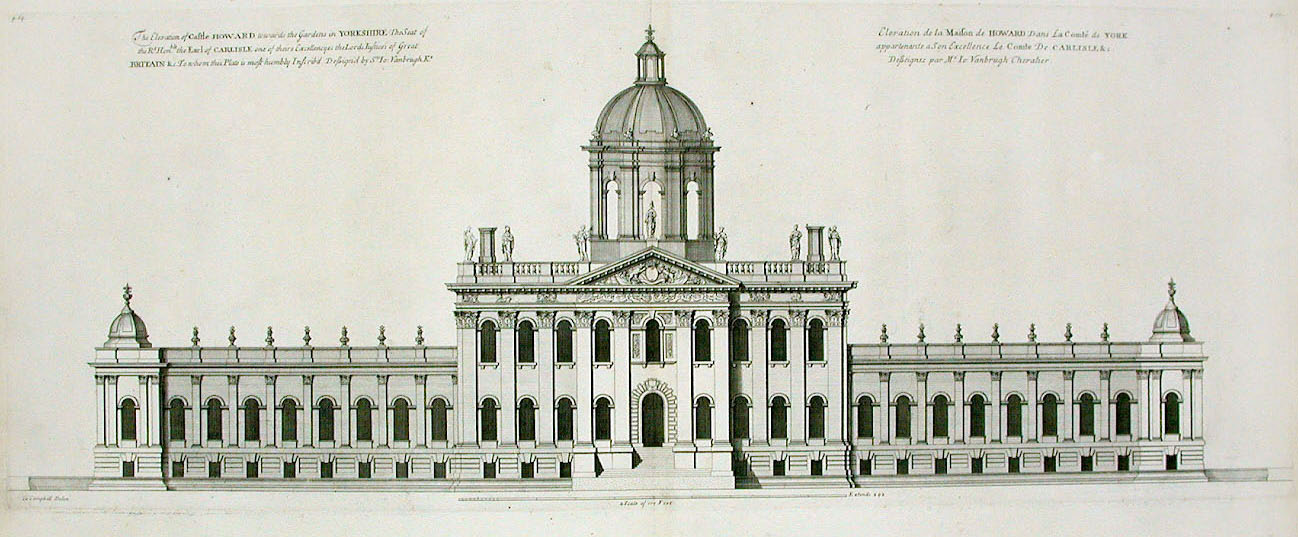
\includegraphics[width=\textwidth]{chapters/60-gruppen/images/castle.jpeg}
\caption{Das Castle Howard in Yorkshire war in dieser ausgeprägt symmetrischen
Form geplant, wurde dann aber in modifizeirter Form gebaut.
Messungen zwischen Punkten in der rechten Hälfte des Bildes
ergeben die gleichen Werte wie Messungen entsprechenden Strecken
in der linken Hälfte, was den Begriff Symmetrie rechtfertigt.
\label{buch:lie:bild:castlehoward}}
\end{figure}
In der Physik wird dem Begriff der Symmetrie daher auch eine erweiterte
Bedeutung gegeben.
Jede Transformation eines Systems, welche bestimmte Grössen nicht
verändert, wird als Symmetrie bezeichnet.
Die Gesetze der Physik sind typischerweise unabhängig davon, wo man den
den Nullpunkt der Zeit oder das räumlichen Koordinatensystems ansetzt,
eine Transformation des Zeitnullpunktes oder des Ursprungs des
Koordinatensystems ändert daher die Bewegungsgleichungen nicht, sie ist
eine Symmetrie des Systems.

Umgekehrt kann man fragen, welche Symmetrien ein System hat.
Da sich Symmetrien zusammensetzen und umkehren lassen, kann man in davon
ausgehen, dass die Symmetrietransformationen eine Gruppe bilden.
Besonders interessant ist dies im Falle von Transformationen, die
durch Matrizen beschrieben weren.
Eine unter der Symmetrie erhaltene Eigenschaft definiert so eine
Untergruppe der Gruppe $\operatorname{GL}_n(\mathbb{R})$ der
invertierbaren Matrizen.
Die erhaltenen Eigenschaften definieren eine Menge von Gleichungen,
denen die Elemente der Untergruppe genügen müssen.
Als Lösungsmenge einer Gleichung erhält die Untergruppe damit eine
zusätzliche geometrische Struktur, man nennt sie eine differenzierbare
Mannigfaltigkeit.
Dieser Begriff wird im Abschnitt~\ref{buch:subsection:mannigfaltigkeit}
eingeführt.
Es wird sich zum Beispiel zeigen, dass die Menge der Drehungen der
Ebene mit den Punkten eines Kreises parametrisieren lassen,
die Lösungen der Gleichung $x^2+y^2=1$ sind.

Eine Lie-Gruppe ist eine Gruppe, die gleichzeitig eine differenzierbare
Mannigfaltigkeit ist.
Die Existenz von geometrischen Konzepten wie Tangentialvektoren
ermöglicht zusätzliche Werkzeuge, mit denen diese Gruppe untersucht
und verstanden werden können.
Ziel dieses Abschnitts ist, die Grundlagen für diese Untersuchung zu
schaffen, die dann im Abschnitt~\ref{buch:section:lie-algebren}
durchgeführt werden soll.

\subsection{Algebraische Symmetrien
\label{buch:subsection:algebraische-symmetrien}}
Mit Matrizen lassen sich Symmetrien in einem geometrischen Problem
oder in einem physikalischen System beschreiben.
Man denkt dabei gerne zuerst an geometrische Symmetrien wie die
Symmetrie unter Punktspiegelung oder die Spiegelung an der $x_1$-$x_2$-Ebene,
wie sie zum Beispiel durch die Abbildungen
\[
\mathbb{R}^3\to\mathbb{R}^3 : x\mapsto -x
\qquad\text{oder}\qquad
\mathbb{R}^3\to\mathbb{R}^3 :
\begin{pmatrix}x_1\\x_2\\x_3\end{pmatrix}
\mapsto
\begin{pmatrix}-x_1\\x_2\\x_3\end{pmatrix}
\]
dargestellt werden.
Beide haben zunächst die Eigenschaft, dass Längen und Winkel und damit
das Skalarprodukt erhalten sind.
Diese Eigenschaft allein erlaubt aber noch nicht, die beiden Transformationen
zu unterscheiden.
Die Punktspiegelung zeichnet sich dadurch aus, das alle Geraden und alle
Ebenen durch den Ursprung auf sich selbst abgebildet werden.
Dies funktioniert für die Ebenenspiegelung nicht, dort bleibt nur die
Spiegelungsebene (die $x_1$-$x_2$-Ebene im vorliegenden Fall) und
ihre Normale erhalten.
Die folgenden Beispiele sollen zeigen, wie solche Symmetriedefinitionen
auf algebraische Bedingungen an die Matrixelemente führen.


\subsection{Manningfaltigkeiten
\label{buch:subsection:mannigfaltigkeit}}

\subsection{Der Satz von Noether
\label{buch:subsection:noether}}







